%% pdflatex
\documentclass[10pt]{beamer}
%% \usepackage{upgreek}
%% \usepackage{hyperref}
%% Fonts
\usepackage{multicol}
\usepackage{mathabx}
\usepackage[scaled]{helvet}
\usepackage{lmodern}
\usepackage{eulervm}
\usefonttheme[onlymath]{serif}
\usefonttheme{professionalfonts}
\usefonttheme{structurebold}
\hypersetup{backref}
\usepackage{bm}
%% Color & Theme
\definecolor{SUblue}{RGB}{0,0,180}
\usecolortheme[RGB={0,0,180}]{structure}
\usetheme{Boadilla}
\setbeamertemplate{navigation symbols}{}
\setbeamerfont{title}{size=\large}
\setbeamerfont{frametitle}{size=\large}
\setbeamerfont{framesubtitle}{size=\large, shape =$\color{violet}{\looparrowdownright}~$}
\setbeamercolor{title}{fg=white, bg= SUblue!75!green}
\setbeamercolor{framesubtitle}{fg=violet}

\title[Multivariate Surface Regression]{{\textbf{Efficient Bayesian
      Multivariate Surface Regression}}}

\author[Feng Li]{\includegraphics[height=2cm]{cufelogo}\\
\vspace{0.5cm}\textbf{Feng Li}\\\texttt{feng.li@cufe.edu.cn}}
\institute[StatMath, CUFE]{\footnotesize{\textbf{School of Statistics and
      Mathematics\\ Central University of Finance and Economics}}}
\date{}

% \author[Feng Li]{\\\vspace{0.7cm}\textbf{Feng Li}  \\\vspace{0.2cm}
%   \textbf{\footnotesize{(jointly with Mattias Villani)}}}
% \institute[Stockholm University]{\footnotesize{\textbf{Department of
%       Statistics, Stockholm University}}}
% \date{\color{SUblue}{ \textbf{Feb, 2012}}}

\begin{document}
%% Title page
\begin{frame}[plain]
  \titlepage
\end{frame}

\section*{Outline of the talk}
\begin{frame}
  \frametitle{Outline of the talk}
  \tableofcontents
\end{frame}

%%%%%%%%%%%%%%%%%%%%%%%%%%%%%%%%%%%%%%%%%%%%%%%%%%%%%%%%%%%%%%%%%%%%%%%%%%%%%%

\section{Introduction to flexible regression models}
\begin{frame}
  \frametitle{Flexible regression models}
  \framesubtitle{Introduction}
  \begin{itemize}
  \item Flexible models of the regression function $E(y|x)$ has been an active research field
    for decades.
  \item Attention has shifted from kernel regression methods to spline-based models.
  \item Splines are regression models with flexible mean functions.
  \item Example: a simple spline regression with only one explanatory variable with truncated linear
    basis function can be like this
    \[y = {\alpha _0} + {\alpha _1}x + {\beta _1}{\left( {x - {\xi _1}} \right)_ + } + ... +
    {\beta _q}{\left( {x - {\xi _q}} \right)_ + } + \varepsilon \]
    where
    \begin{itemize}
    \item $(x-\xi_i)_+$ are called the basis functions,
    \item $\xi_i$ are called knots (the location of the basis function).
    \end{itemize}
    % \item Are splines any good?
    %   \begin{itemize}
    %   \item determine the points of flexibility of the fitted regression function
    %   \item locally polynomial model with continuity at the knots.
    %   \end{itemize}
  \end{itemize}

\end{frame}

% \begin{frame}
%   \frametitle{Introduction}
%   \framesubtitle{Spline example (single covariate with truncated linear bases)}
%   \begin{center}
%     \begin{figure}
%       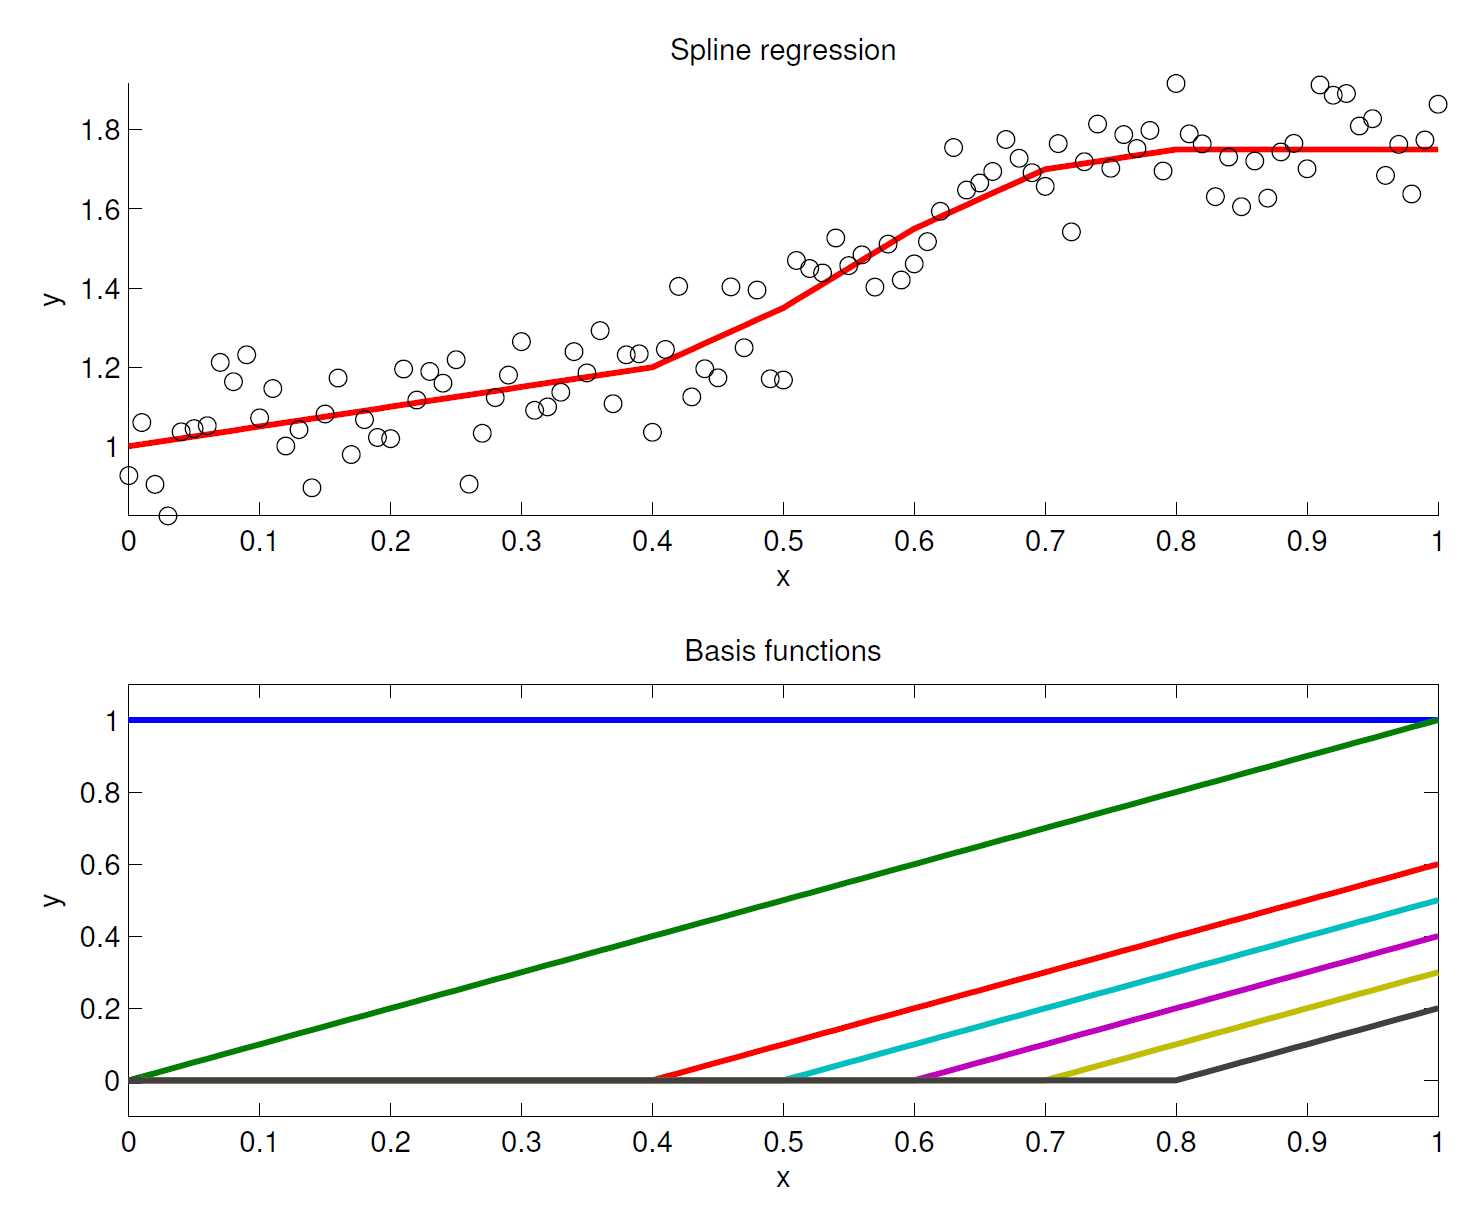
\includegraphics[width=9.5cm]{spline1.png}
%     \end{figure}
%   \end{center}
% \end{frame}

\begin{frame}
  \frametitle{Flexible regression models}
  \framesubtitle{Spline example (single covariate with thinplate bases)}
  \begin{center}
    \begin{figure}
      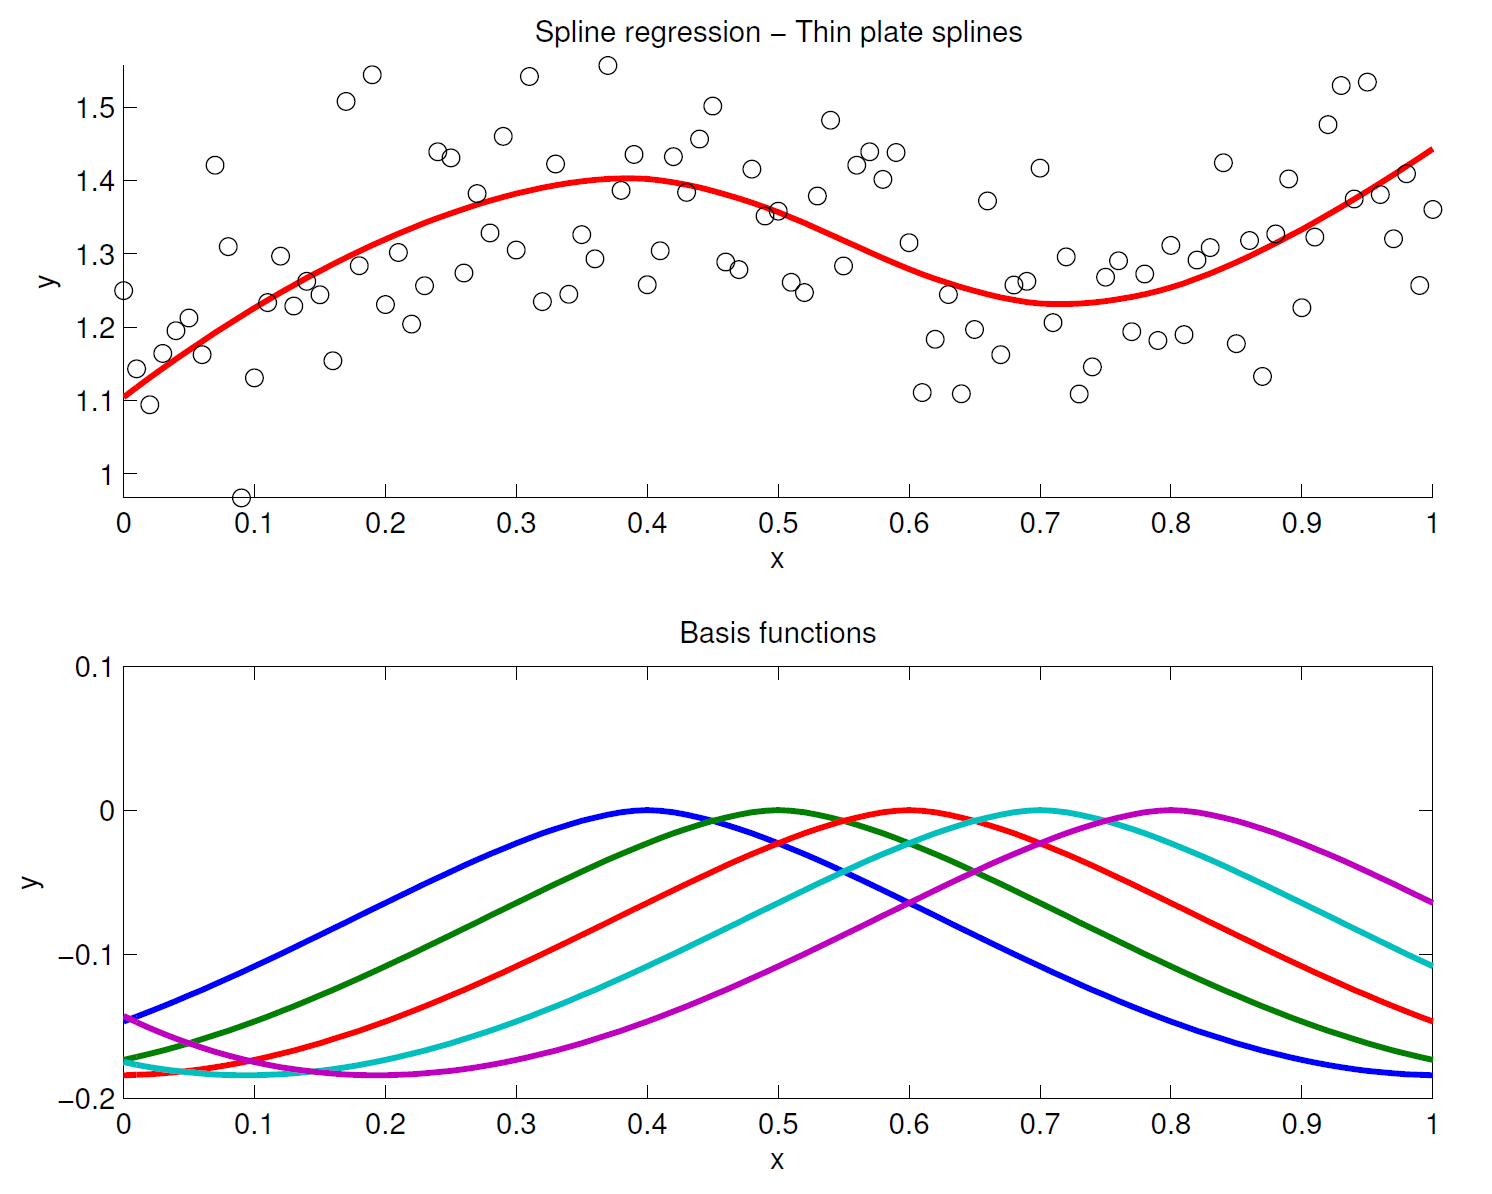
\includegraphics[width=9.5cm]{spline2.png}
    \end{figure}
  \end{center}
\end{frame}

\begin{frame}
  \frametitle{Flexible regression models}
  \framesubtitle{Spline regression with multiple covariates}
  \begin{itemize}
  \item Additive spline model
    \begin{itemize}
    \item Each knot $\xi_{j.}$ (scaler) is connected with only one covariate
      \[y = {\alpha_0} + {\alpha _1}{x_1} + ...+{\alpha _q}{x_q} + \left[ \sum
        \limits_{j_1=1}^{m_1} \beta_{j_1} f\left( {{x_1},{\xi _{j_1}}}
        \right) + ... + \sum \limits_{j_q=1}^{m_q} \beta_{j_q} f\left( {{x_q},{\xi _{j_q}}} \right)\right] + \varepsilon \]
    \item Good and simple if you know there is no interactions in the data a priori.
    \end{itemize}
  \item Surface spline model
    \begin{itemize}
    \item Each knot $\bm{\xi}_j$ (vector) is connected with more than one covariate
      \[y = {\alpha _0} + {\alpha _1}{x_1} + ...+{\alpha _q}{x_q} + \left[ \sum
        \limits_{j=1}^{m}  \beta_j g\left(
          {{x_1},...{x_q},{\bm{\xi} _j}} \right) \right]
      + \varepsilon \]
    \item A popular choice of $g\left( {{x_1},...{x_q},{\bm{\xi} _j}} \right)$ can be
      e.g. the multi-dimensional thinplate spline
      \[g\left( {{x_1},...{x_q},{\bm{\xi} _j}} \right) = {\left\| {\bm{x} - \bm{\xi}_j
          } \right\|^2}\ln \left\| {\bm{x} - \bm{\xi}_j } \right\|\]
    \item Can handle the interactions but the model complexity increase
      dramatically with the interactive knots.
    \end{itemize}

  \end{itemize}
\end{frame}

%\section{The challenges}
\begin{frame}
  \frametitle{The challenges}
  %% \framesubtitle{The model}
  \begin{itemize}
  \item How many knots are needed?
    \begin{itemize}
    \item Too few knots lead to a bad approximation; too many knots yield
      overfitting.
    \end{itemize}
  \item Where to place those knots?
    \begin{itemize}
    \item Equal spacing for the additive model,
    \item which is obviously not efficient with the surface model.
    \end{itemize}
  \item Common approaches to the two problems:
    \begin{itemize}
    \item place enough many knots and use variable selection to pick up useful
      ones.
      \begin{itemize}
      \item not truly flexible
      \end{itemize}
    \item use reversible jump MCMC to move among the model spaces with different
      numbers of knots
      \begin{itemize}
      \item very sensitive to the prior and not computational efficient
      \end{itemize}
    \item clustering the covariates to select knots
      \begin{itemize}
      \item does not use the information from the responses
      \end{itemize}
    \end{itemize}
  \item How to choose between additive spline and surface spline?
    \begin{itemize}
    \item NA
    \end{itemize}
  \end{itemize}
\end{frame}

\section{The multivariate surface model}
\begin{frame}
  \frametitle{The multivariate surface model}
  \framesubtitle{The model}
  \begin{itemize}
  \item The multivariate surface model consists of three different components,
    {\color{blue}\emph{linear}}, {\color{blue}\emph{surface}} and
    {\color{blue}\emph{additive}} as
    \[\begin{gathered}
      \bm{Y}=\bm{X}_o\bm{B}_o+
      \bm{X}_s(\xi_s)\bm{B}_s+\bm{X}_a(\xi_a)\bm{B}_a + \bm{E}.
    \end{gathered}\]
  \item We treat the knots $\xi_i$ as unknown parameters and let them move
    freely.
    \begin{itemize}
    \item A model with a minimal number of free knots outperforms model with lots
      of fixed knots.
    \end{itemize}
  \item For notational convenience, we sometimes write model in compact form
    \[
    \bm{Y}=\bm{X}\bm{B}+\bm{E},
    \]
    where $\bm{X}=[\bm{X}_{o},\bm{X}_{s},\bm{X}_{a}]$ and
    $\bm{B}=[{\bm{B}_{o}}',{\bm{B}_{s}}',{\bm{B}_{a}}']'$ and $\bm{E}\sim \bm{N}_p(\bm{0},~\bm{\Sigma})$
  \end{itemize}
\end{frame}

\begin{frame}
  \frametitle{The multivariate surface model}
  \framesubtitle{The prior}
  \begin{itemize}
  \item Conditional on the knots, the prior for $\bm{B}$ and
    $\bm{\Sigma}$ are set as
    \[
    \begin{split}
      \mathrm{vec}\bm{B}_i |\bm{\Sigma},~\bm{\lambda}_i &\sim \bm{N}_q\left[
        \mu _i, ~\bm{\Lambda}_i^{1/2} \bm{\Sigma} \bm{\Lambda}_i^{1/2} \otimes
        \bm{P}_i^{-1}
      \right], ~i\in \{o,s,a \},\\
      \bm{\Sigma} &\sim \bm{IW} \left[n_0 \bm{S}_0,~n_0\right],
    \end{split}
    \]
    \begin{itemize}

    \item $\bm{\Lambda}_i=diag(\bm{\lambda}_i)$ are called the shrinkage parameters,
      which is used for overcome overfitting through the prior.
    \item If $\bm{P}_i=\bm{I}$, can
      prevent singularity problem, like the ridge regression estimate.

    \item If $\bm{P}_i=\bm{X}_i'\bm{X}_i$: use the covariates
      information, also a compressed version of least squares estimate when
      $\bm{\lambda}_i$ is large.
    \end{itemize}
  \item The shrinkage parameters are estimated in MCMC
    \begin{itemize}
    \item A small $\bm{\lambda}_{i}$ shrinks the variance of the conditional posterior
      for $\bm{B}_i$
    \item It is another approach to selection important variables (knots) and
      components.
    \end{itemize}
  \item We allow to mixed use the two types priors ( $\bm{P}_i=\bm{I}$,
    $\bm{P}_i=\bm{X}_i'\bm{X}_i$) in different components in order to take the both
    the advantages of them.
  \end{itemize}
\end{frame}

\begin{frame}
  \frametitle{The multivariate surface model}
  \framesubtitle{The Bayesian posterior}
  \begin{itemize}
  \item The posterior distribution is conveniently decomposed as
    \[
    p(\bm{B},\bm{\Sigma},\bm{\xi},\bm{\lambda}|\bm{Y},\bm{X})=p(\bm{B}|\bm{\Sigma},\bm{\xi},\bm{\lambda},\bm{Y},\bm{X})p(\bm{\Sigma}|\bm{\xi},\bm{\lambda},\bm{Y},\bm{X})p(\bm{\xi},\bm{\lambda}|\bm{Y},\bm{X}).
    \]
  \item Hence $p(\bm{B}|\bm{\Sigma},\bm{\xi},\bm{\lambda},\bm{Y},\bm{X})$ follows
    the multivariate normal distribution according to the conjugacy;
  \item When $p=1$, $p(\bm{\Sigma}|\bm{\xi},\bm{\lambda},\bm{Y},\bm{X})$ follows the inverse Wishart distribution
    \[
    \bm{IW} \left[n_0+n, \left\{{n_0}{\bm{S}_0} + n \tilde {\bm{S}} +
        \sum\limits_{i \in \{ o,s,a\} } {{\bm{\Lambda}}_i^{-1/2}({{\tilde
              {\bm{B}}_i}} - {\bm{M}_i})'{\bm{P}_i}({{\tilde {\bm{B}}}_i} -
          {\bm{M}_i}){\bm{\Lambda}}_i^{ - 1/2}}\right\} \right]
    \]
  \item When $p \geq 2$, no closed form of
    $p(\bm{\Sigma}|\bm{\xi},\bm{\lambda},\bm{Y},\bm{X})$, the above result is a
    very accurate approximation. Then the marginal posterior of $\bm{\Sigma}$,
    $\bm{\xi}$ and $\bm{\lambda}$ is
    \[\begin{split}
      p\left(\bm{\Sigma}, {\bm{\xi} ,\bm{\lambda} |\bm{Y},\bm{X}} \right) =
      &c\times p(\bm{\xi},\bm{\lambda})\times {|
        {{\bm{\Sigma}_{\bm{\beta}} }} |^{ - 1/2}}{| \bm{\Sigma} |^{ - (n + {n_0} + p +
          1)/2}}{| {{\bm{\Sigma}_{\bm{\tilde
                \beta} }}} |^{ - 1/2}}\\
      &\times \exp \left\{ { - \frac{1}{2}\left[ {\mathrm{tr}{\bm{\Sigma}^{ - 1}}\left(
                {{n_0}{\bm{S}_0} + n\bm{\tilde S}} \right) + \left( {\bm{\tilde \beta} -
                  \bm{\mu} } \right)'{\bm{\Sigma}_{\bm{\beta}}^{-1} }\left( {\bm{\tilde \beta} - \bm{\mu} }
              \right)} \right]} \right\}
    \end{split}\]
  \end{itemize}
\end{frame}

% \section{The MCMC algorithm}
\begin{frame}
  \frametitle{The MCMC algorithm}
  \framesubtitle{Metropolis-Hastings within Gibbs}
  \begin{itemize}
  \item The coefficients ($\bm{B}$) are directly sampled from normal distribution.
  \item We update covariance ($\bm{\Sigma}$), all knots ($\bm{\xi}$) and shrinkages ($\bm{\lambda}$) jointly by using
    Metropolis-Hastings within Gibbs.
  \item  The proposal density for $\bm{\Sigma}$ is the inverse Wishart
    density on previous slide.
  \item The proposal density for $\bm{\xi}$ and $\bm{\lambda}$ is a multivariate \emph{t}-density with $\nu>2$ df,
    \[
    \bm{\theta}_{p}|\bm{\theta}_{c}\sim\bm{MVT}\left[\bm{\hat{\theta}},~\left.-\left(\frac{\partial^{2}\ln
            p(\bm{\theta}|\bm{Y})}{\partial\bm{\theta}\partial\bm{\theta}^{\prime}}\right)^{-1}\right\vert
      _{\bm{\theta}=\bm{\hat{\theta}}},~\nu\right],
    \]
     where $\bm{\hat{\theta}}$ is obtained by $R$ steps ($R\leq 3$) Newton's
      iterations during the proposal with analytical gradients for matrices.

    \item The analytical gradients are very complicated and we have
      implemented it in an efficient way (\textbf{the key!}).

  \end{itemize}
\end{frame}

% \begin{frame}
%   \frametitle{The MCMC algorithm}
%   \framesubtitle{Computational remarks}
%   \begin{itemize}
%   \item It a complicated model with a lot of parameters:
%     \begin{itemize}
%     \item e.g., a 10 covariates, univariate response with 50 knots in both additive
%       and surface components need $10\times 50 + 1\times 50 + 110 + 1 = 661$
%       parameters.
%     \end{itemize}

%   \item The MCMC implementations are straightforward.

%   \item We allow the parameters to be updated via:
%     \begin{itemize}
%     \item parallel mode for small datasets,
%     \item batched mode for big datasets.
%     \end{itemize}

%   \end{itemize}
% \end{frame}

% \section{Simulation study}

% \begin{frame}[plain]
%   \begin{multicols}{3}
%     \large{\color{SUblue} \textbf{Simulation study}}

%     \begin{itemize}
%     \item \tiny{We randomly generate 100 datasets with various degrees of nonlinearity
%         ($p=1,~2$, $n = 200, ~1000$). \\Covariates: Mixture of multivariate normal with five
%         components; \\Bases: Five true bases from the covariates.}
%     \item \tiny{For each dataset we fit with the fixed knots model for 5,
%         10, 15, 20, 25 and 50 surface knots, and also the free knots model for 5, 10, and 15 surface
%         knots.}
%     \item \tiny{The results show the free knots model outperforms the fixed knots
%         model in the large majority of the datasets. This is particularly true when
%         the data are strongly nonlinear.}
%       \vspace{0.3cm}
%       \hrule
%     \item \tiny{Some results from the simulation {\color{blue} $\bm{\rightarrow}$}}
%     \item \tiny{The norm of the predictive multivariate residuals ($p=2$) against
%         the distance between the testing covariates $\bm{x}$ (randomly selected
%         covariates space, therefore out-of-sample) and DGP sample mean.}
%     \item \tiny{The residuals from vertical bars above the zero line is from
%         the model with 15 fixed surface knots.}
%     \item \tiny{The residuals from vertical bars below the zero line is from
%         the model with 5 free surface knots.}
%     \end{itemize}

%     \begin{center}
%       \begin{figure}
%         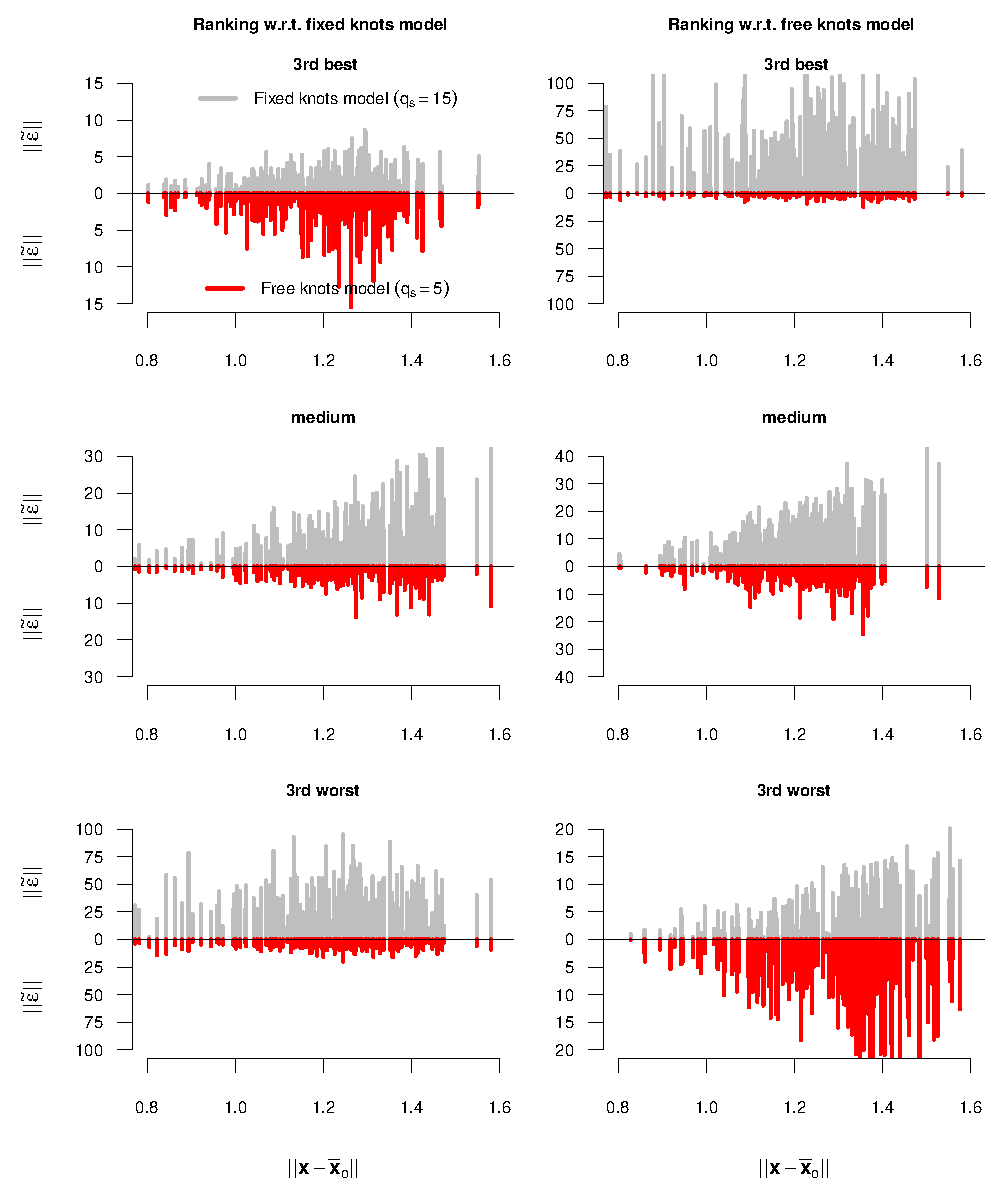
\includegraphics[height=\textheight]{SimResidPlot.eps}
%       \end{figure}
%     \end{center}
%   \end{multicols}
% \end{frame}

\section{Application to firm leverage data}
\begin{frame}
  \frametitle{Application to firm leverage data}
  \framesubtitle{The data}
  \vspace{0.25cm}
  \scalebox{0.65}{
    \begin{tabular}{rl}
      \textbf{leverage ($Y$):} &total debt/(total debt+book value of equity), 4405 observations;\\
      \textbf{tang:} & tangible assets/book value of total assets;\\
      \textbf{market2book:} &(book value of total assets - book value of equity +
      market value of equity) / book value of total assets;\\
      \textbf{logSales:} &logarithm of sales;\\
      \textbf{profit:} &(earnings before interest, taxes, depreciation, and amortization) /
      book value of total assets.    \\
    \end{tabular}}
  \vspace{0.25cm}
  \begin{center}
    \begin{figure}
      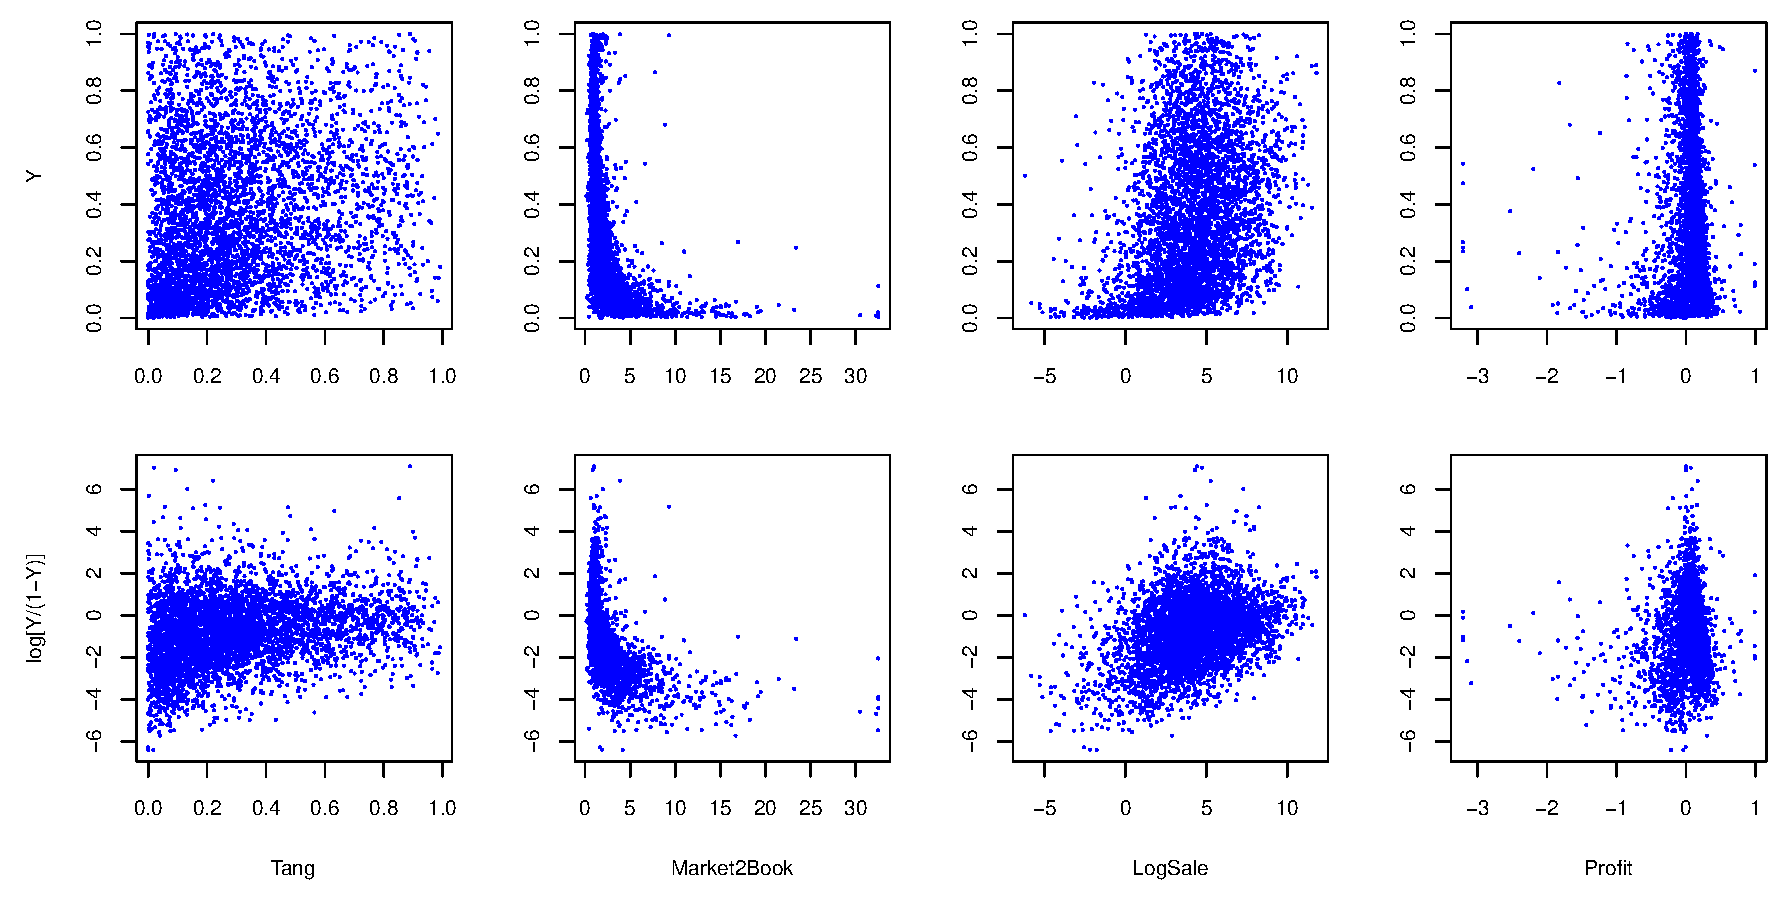
\includegraphics[width=\textwidth]{Rajanscatter.eps}
    \end{figure}
  \end{center}
\end{frame}

\begin{frame}[plain]
  \begin{multicols}{2}
    \begin{center}
      \begin{figure}
        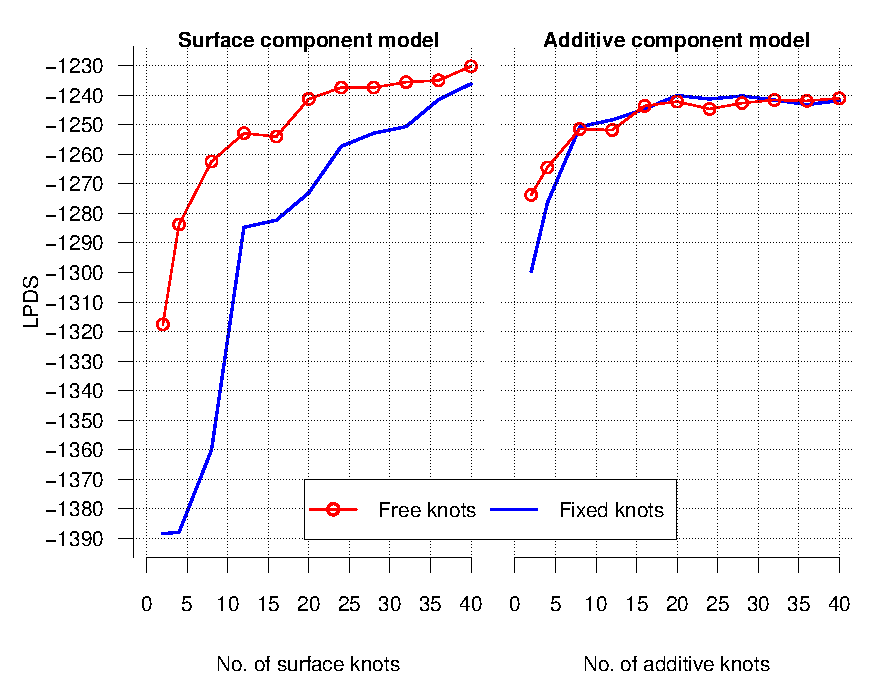
\includegraphics[width=0.5\textwidth]{RajanLPDS_SurfaceBesideAdditive}
      \end{figure}
    \end{center}
    \begin{enumerate}
    \item [$\uparrow$] \tiny{Models with only surface or additive components}
    \item [$\rightarrow$] \tiny{Model with both additive and surface
        components.}
    \item [LPDS] \tiny {Log predictive density score which is defined as
        \[
        \begin{split}
          LPDS=&\frac{1}{D}\sum\nolimits_{d=1}^{D}\ln
          p(\tilde{\bm{Y}}_{d}|\tilde{\bm{Y}}_{-d},\bm{X})\\
          =&\int\!\prod\nolimits_{i\in\tau_{d}}p(\bm{y}_{i}|\bm{\theta},
          \bm{x}_{i})p(\bm{\theta}|\tilde{\bm{Y}}_{-d})\mathrm{d}\bm{\theta},
        \end{split}
        \]
        and $D=5$ in the cross-validation.}
    \end{enumerate}

    \begin{center}
      \begin{figure}
        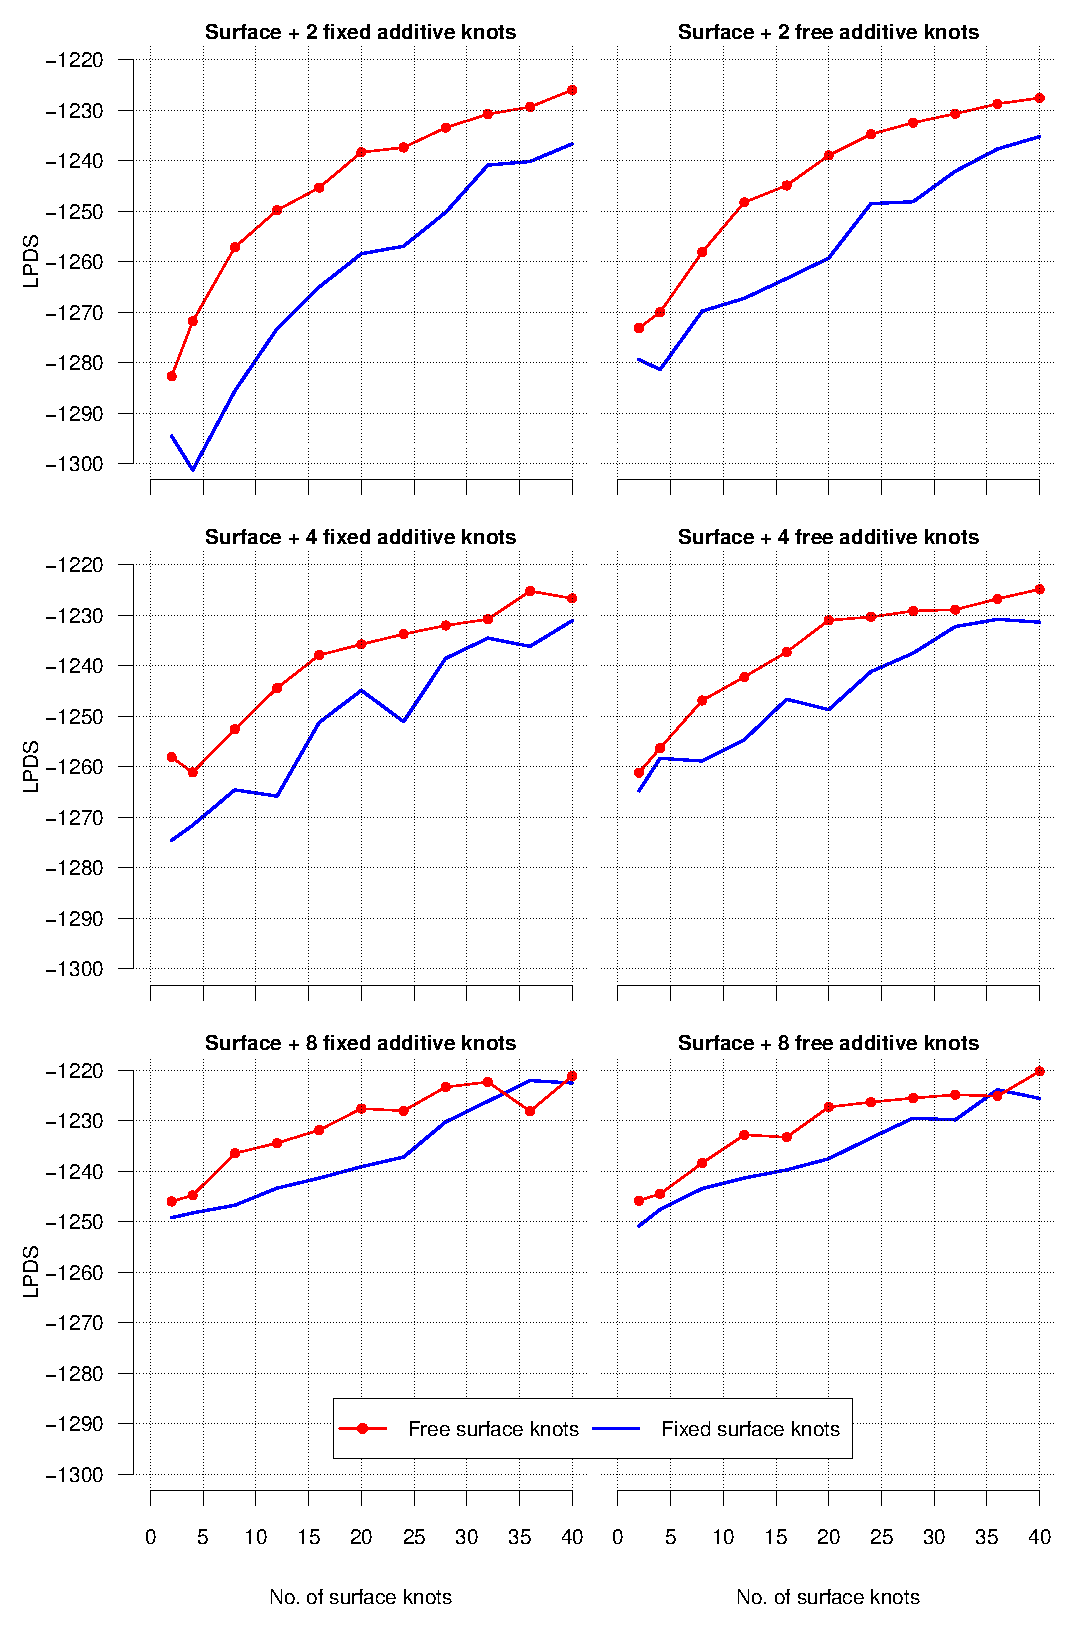
\includegraphics[height=\textheight]{RajanLPDS_SurfacePlusAdditive}
      \end{figure}
    \end{center}
  \end{multicols}
\end{frame}

% \begin{center}
%   \begin{figure}
%     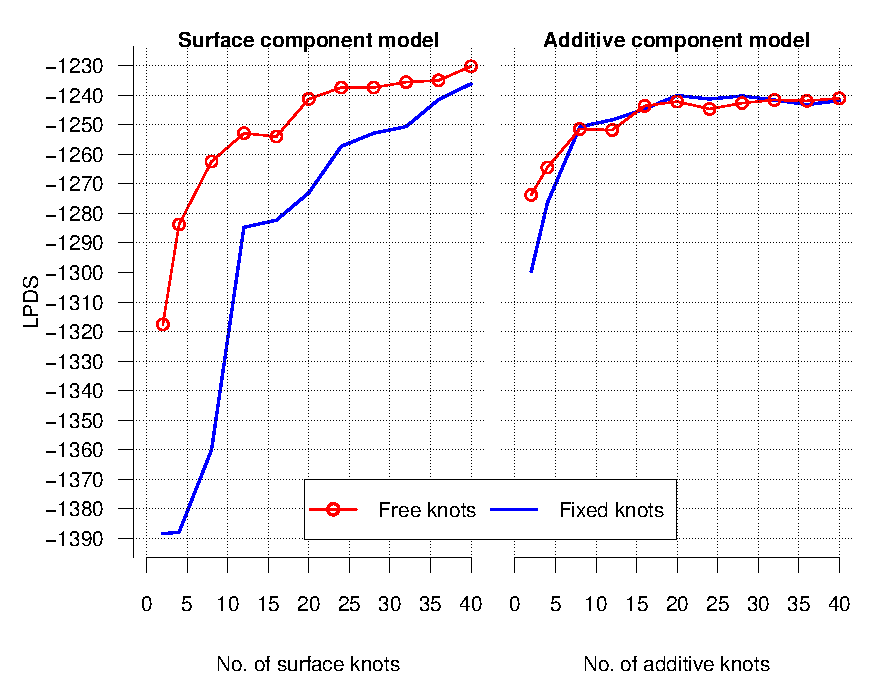
\includegraphics[width=0.5\textwidth]{RajanLPDS_SurfaceBesideAdditive} 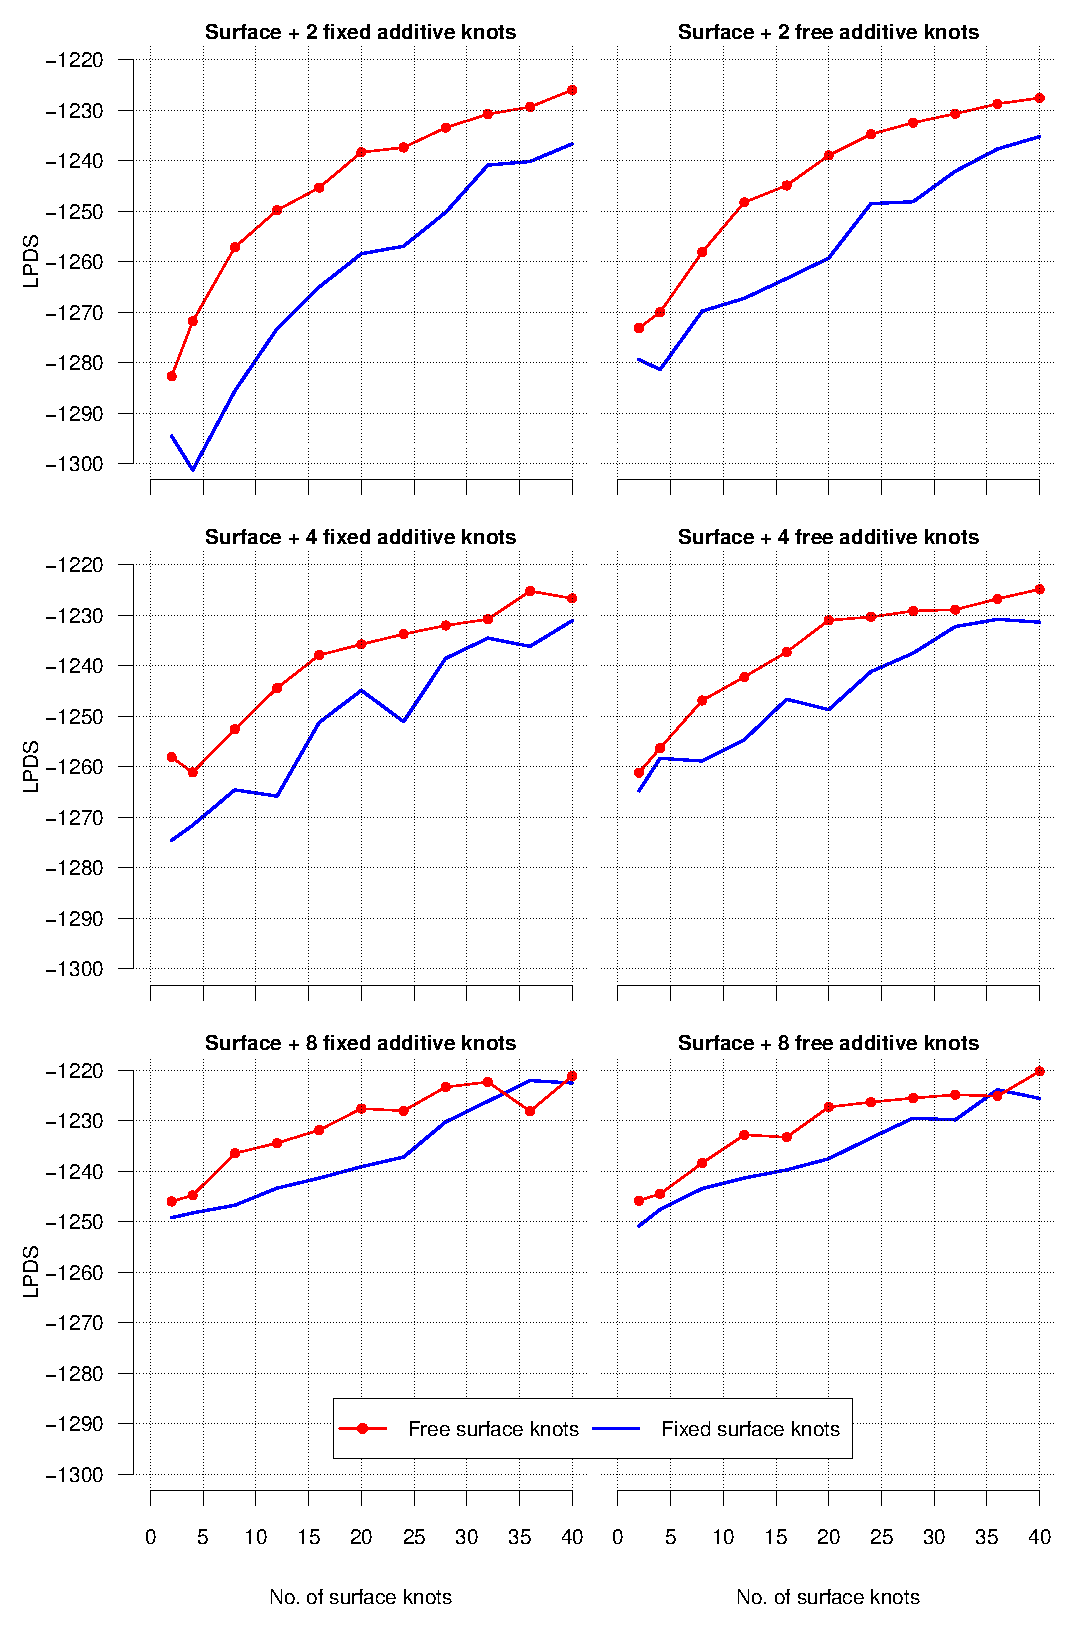
\includegraphics[height=\textheight]{RajanLPDS_SurfacePlusAdditive}
%   \end{figure}
% \end{center}
% \end{frame}

\begin{frame}[plain]
  %% \frametitle{Application to firm leverage data}
  \framesubtitle{The posterior locations for knots}
  \begin{center}
    \begin{figure}
      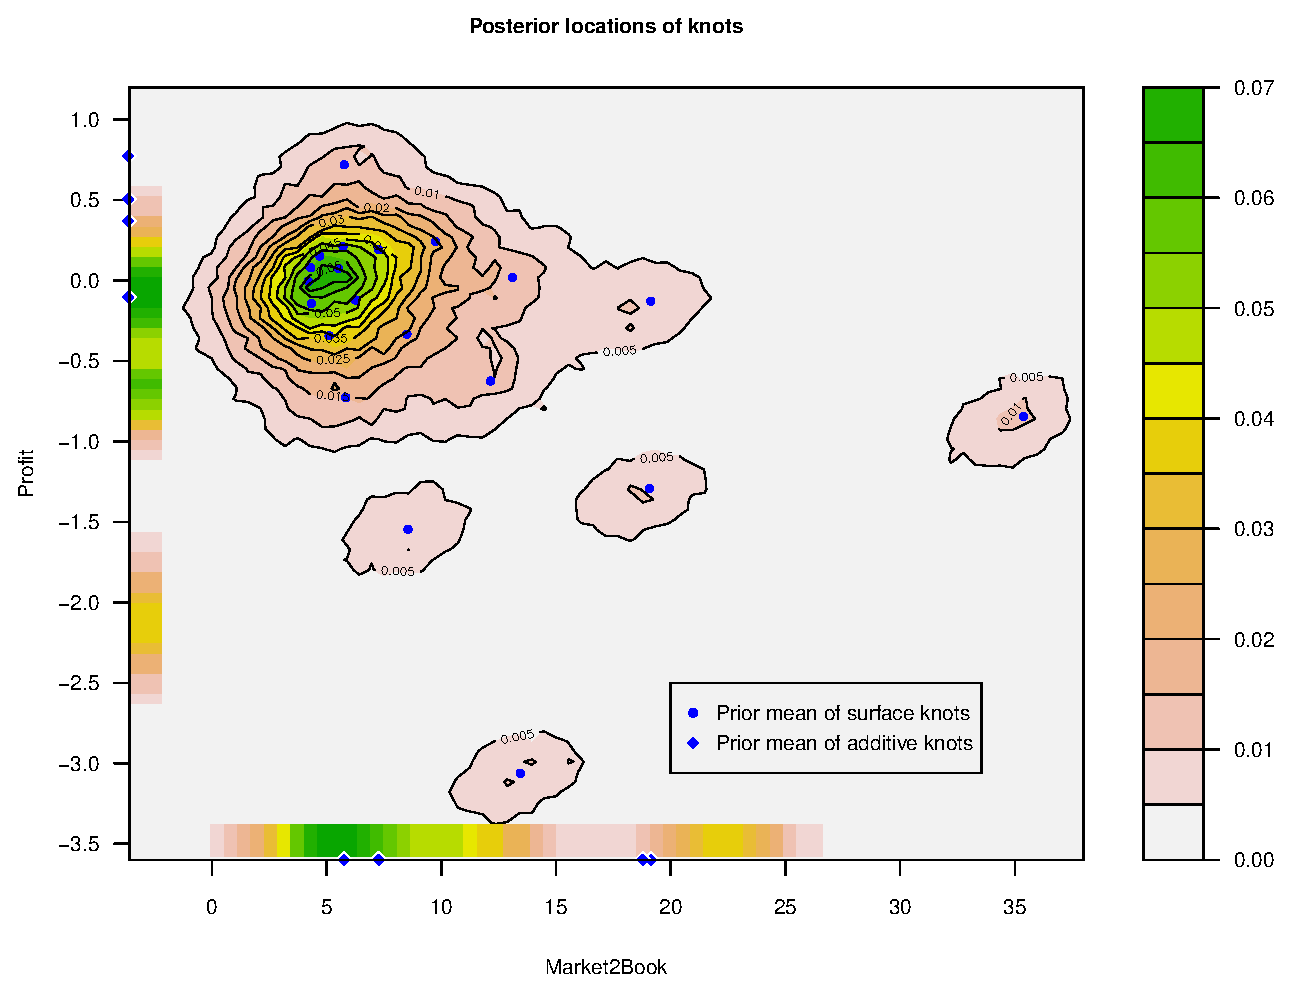
\includegraphics[height=\textheight]{RajanPostKnots.eps}
    \end{figure}
  \end{center}
\end{frame}

\begin{frame}
  \frametitle{Application to firm leverage data}
  \framesubtitle{Posterior mean surface(left) and standard deviation(right)}
  \begin{center}
    \begin{figure}
      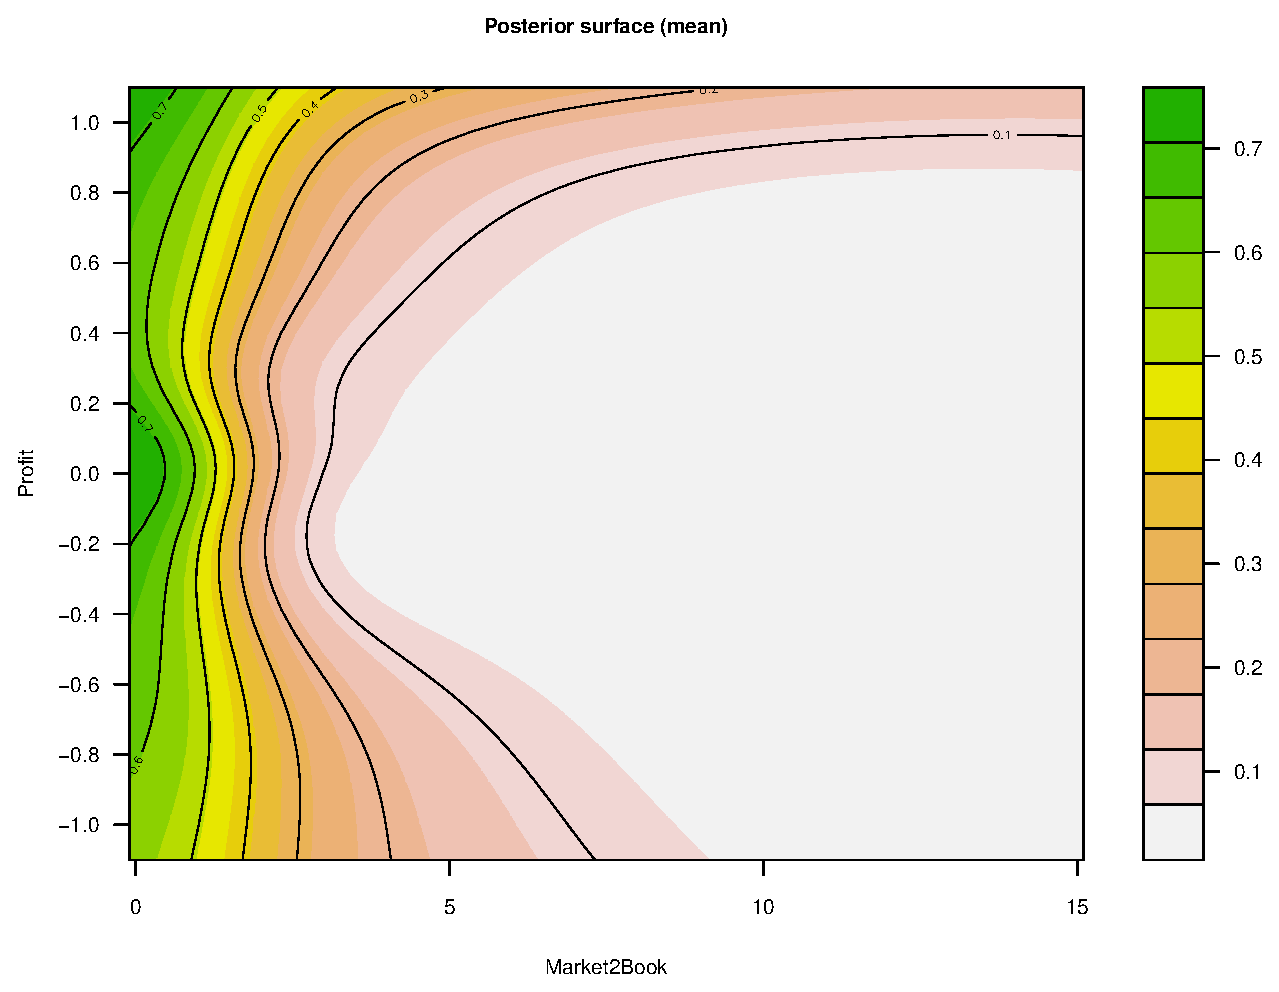
\includegraphics[width=0.5\textwidth]{RajanPostMean.eps}~~~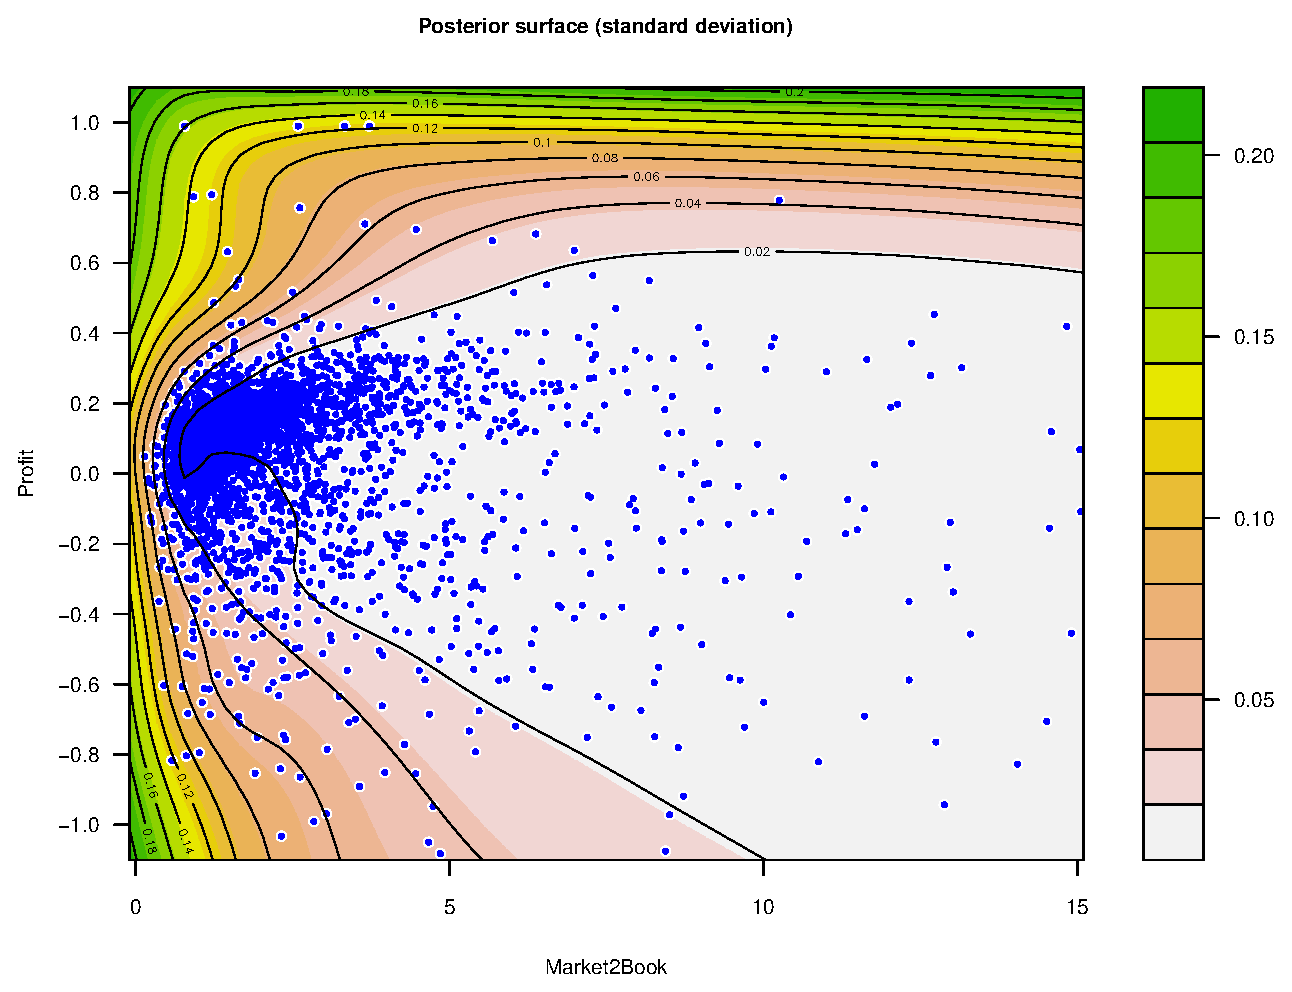
\includegraphics[width=0.5\textwidth]{RajanPostSD.eps}
    \end{figure}
  \end{center}
\end{frame}

\section{Extensions and future work}
\begin{frame}
  \frametitle{Extensions and future work}
  \begin{itemize}
  \item The model and the methods we used are very general.
  \item It is easy to generalize the model to GLM framework.
  \item Variable selection is possible for knots.
  \item Dirichlet precess prior can be plugged into the model when
    heteroscedasticity is the problem.
  \item And the copula...
  \end{itemize}
\end{frame}

\begin{frame}[plain]
  \begin{center}
    \begin{figure}
      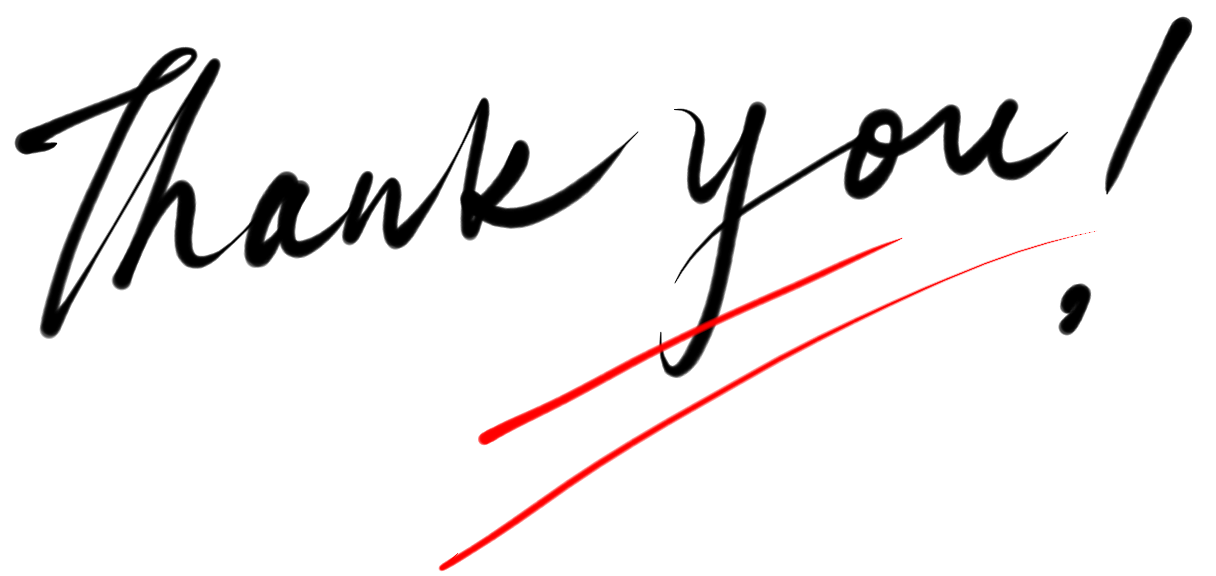
\includegraphics[height=3.0cm]{thankyou.png}
    \end{figure}
  \end{center}
\end{frame}
\end{document}